\section{Decider for halting segment}\label{sec:halting-segment}

\begin{figure}
  \centering
  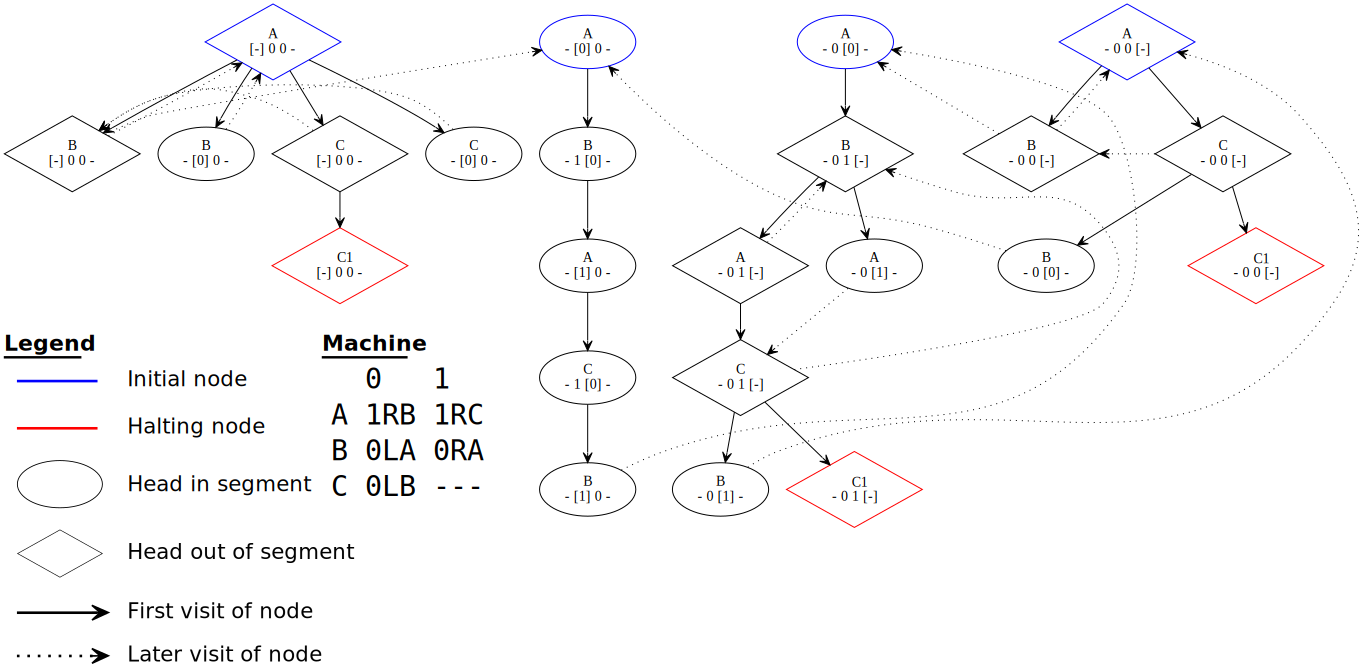
\includegraphics[width=1\textwidth]{halting-segment.pdf}
  \caption{Halting segment graph for the 3-state machine \url{https://bbchallenge.org/1RB1RC_0LA0RA_0LB---} and segment size 2, see Definition~\ref{def:hs-graph}. Nodes of this graph correspond to configurations of the machine on a finite segment (here, of size 2). Nodes where the machine's head is within the segment (circle shape) only one have child corresponding to the next step of the machine and not where the head is outside of the segment (diamond shape) may have multiple children corresponding to all the theoretically possible ways (deduced from the machine's transition table) that the machine can enter the segment back or continue to stay out of it. In order to improve readibility, edges that revisit a node are dotted. The machine presented here does not halt because the halting nodes (red outline) that are reachable from the initial nodes (blue outline) do not cover all the positions of the segment (there is no halting node for any of the two internal positions of the segment), see Theorem~\ref{th:hs:todo}. }
\end{figure}